\documentclass[12pt]{article}
\usepackage[utf8]{inputenc}
\usepackage{float}
\usepackage{amsmath}
\usepackage[hmargin=3cm,vmargin=6.0cm]{geometry}
\topmargin=-2cm
\addtolength{\textheight}{6.5cm}
\addtolength{\textwidth}{2.0cm}
\setlength{\oddsidemargin}{0.0cm}
\setlength{\evensidemargin}{0.0cm}
\usepackage{indentfirst}
\usepackage{amsfonts}
\usepackage{graphicx}
\graphicspath{ {./} }
\begin{document}

\section*{Student Information}

Name : Ahmet Eren Çolak\\

ID : 2587921\\

\section*{Answer 1}
\subsection*{a)}
Size of the Monte Carlo simulation with the significance level $\alpha=0.01$, and amount of error $\varepsilon = 0.02$ is:
\begin{equation*}
	N \geq 0.25 \left(\frac{z_{\alpha/2}}{\varepsilon} \right)^2
\end{equation*}
From the z-table $z_{0.005} = 2.57$
\begin{equation*}
	N \geq 0.25 \left(\frac{2.57}{0.02} \right)^2 = 4128.0625
\end{equation*}
Then $N$ must be at least $4129$.
\subsection*{b)}
Expected value of the random variable $W_a$, weight of an automobile is $\alpha / \lambda$.
\begin{equation*}
	E(W_t) = \frac{190}{0.15} = 1266.67
\end{equation*}

Expected value of the random variable $W_t$, weight of a truck is $\alpha / \lambda$.
\begin{equation*}
	E(W_t) = \frac{110}{0.01} = 11000
\end{equation*}

Random variable representing the total weight of all automobiles that pass over the bridge on a day is $N_a \cdot W_a$ where $N_a$ is a Poisson random variable representing the number of automobiles that pass over the bridge on a day. Since $N_a$ and $W_a$ are independent, $E(N_aW_a) = E(N_a)E(W_a)$

\begin{equation*}
	E(N_a) = \lambda = 50
\end{equation*}
\begin{equation*}
	E(N_aW_a) = E(N_a)E(W_a)=50 \cdot 1266.67 = 63333.5
\end{equation*}

Random variable representing the total weight of all trucks that pass over the bridge on a day is $N_t \cdot W_t$ where $N_t$ is a Poisson random variable representing the number of trucks that pass over the bridge on a day. Since $N_t$ and $W_t$ are independent, $E(N_tW_t) = E(N_t)E(W_t)$

\begin{equation*}
	E(N_t) = \lambda = 10
\end{equation*}
\begin{equation*}
	E(N_tW_t) = E(N_t)E(W_t)=10 \cdot 11000 = 110000
\end{equation*}
\section*{Answer 2}
\begin{center}
	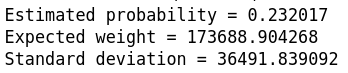
\includegraphics{estimates}
\end{center}

When error rate $\varepsilon = 0.02$ is considered, $\hat{X}$ should be in the interval $(X - X\cdot0.02, X + X \cdot 0.02)$ which is approximately equal to (16986, 17679). Since all estimated values are in this interval, it can be said that estimator $X$ is accurate.
\end{document}
